In order to address the research inquiries posed in~\autoref{sec:research-questions}, it is imperative to first comprehend the subjects and their fundamentals. 

We start by defining the topic areas touched upon by this thesis~(\autoref{sec:defs}), then explain the technologies used within the tool ExpoSE ~(\autoref{sec:defs}), and finally explain the limitations imposed by the engine itself~(\autoref{sec:limits}). 

\section{Definitions}
\label{sec:defs}
To provide an overview of all the topics that will be addressed, we will begin by defining the key components of this thesis and explaining the basics to build upon in the later chapters. 
\subsection{Web Applications}
\label{sec:webapp}
A \textit{web application} has been defined as “a software application, executed by a web server, which responds to dynamic web page requests over HTTP” by the Web Application Security Consortium (WASC) ~\cite{noauthor_web_2012}. 
In simpler terms, a web application is software that runs on a server and users access it through a web browser (like Chrome or Firefox) over the internet.

Typically, the resources and scripts of web applications — such as images, text, or functionalities — are requested by the client, which is the user's computer or device, using a web browser or similar tools. This interaction follows a set of rules known as the API (Application Programming Interface), which specifies what requests can be made and how the server should respond.
The~\autoref{fig:simplified-web-app} illustrates the basic communication process between the client (the user's device), the server (where the application runs), and external services (such as another server).


Most web applications also use a database, which is a structured way of storing data, to keep information consistently available and reliable. For the purposes of this discussion, we assume that the web application has a monolithic architecture. This means that it operates as a single cohesive program on a physical computer, as opposed to being divided into separate parts that run on different cloud services (like AWS, or Amazon Web Services, which offers online computing power without needing dedicated hardware)~\cite{noauthor_serverless_nodate}.
Additionally, we assume the server follows REST (Representational State Transfer) principles, which are guidelines for how web services should operate to enable smooth communication as described by \citet{roy_t_fielding_rest_2008}. 
The web server processes requests that adhere to the HTTP (Hypertext Transfer Protocol) standard, which is the foundational protocol used for transmitting data on the web (ref. ~\autoref{tab:rest_http_methods}).
This adherence ensures that the server and client can operate independently, meaning they can be developed and updated separately without affecting each other\cite{fielding_http_2022}.

\begin{figure}[h]
    \centering
    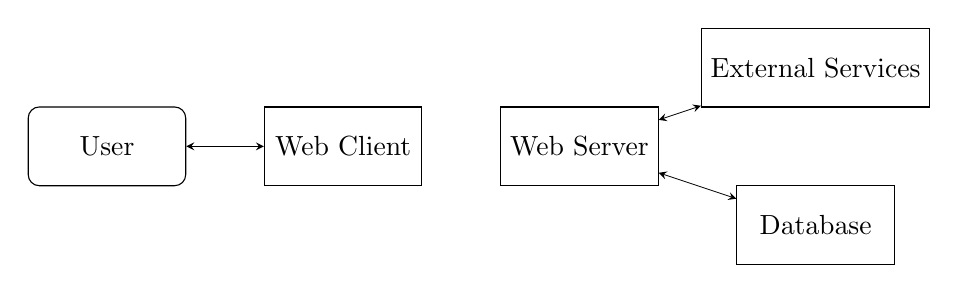
\begin{tikzpicture}[node distance=3cm]
    % Define styles for nodes and arrows
    \tikzstyle{user} = [rectangle, rounded corners, minimum width=2cm, minimum height=1cm, text centered, draw=black]
    \tikzstyle{browser} = [rectangle, minimum width=2cm, minimum height=1cm, text centered, draw=black]
    \tikzstyle{server} = [rectangle, minimum width=2cm, minimum height=1cm, text centered, draw=black]
    \tikzstyle{database} = [rectangle, minimum width=2cm, minimum height=1cm, text centered, draw=black]
    \tikzstyle{external} = [rectangle, minimum width=2cm, minimum height=1cm, text centered, draw=black]
    % Use arrows with both directions
    \tikzstyle{arrow} = [thick, <->, >=stealth]
% Arrow style for double lines

    \tikzset{doubleArrow/.style={thick, <->, >=stealth,
        line width=0.1mm, line cap=round, draw=black
    }}
    % Nodes
    \node (user) [user] {User};
    \node (browser) [browser, right of=user] {Web Client};
    \node (server) [server, right of=browser] {Web Server};
    \node (database) [database, right of=server, yshift=-1cm] {Database};
    \node (external) [external, right of=server, yshift=1cm] {External Services};
    % Arrows (connections)
    \draw  [doubleArrow](user) -- (browser);
    \draw  [doubleArrow](server) -- (database);
    \draw [doubleArrow] (server) -- (external);
    \end{tikzpicture}
    \caption{Structure of a simplified Web Application}
    \label{fig:simplified-web-app}

\end{figure}

\begin{table}[htb]
    \centering
    \begin{tabular}{@{}lll@{}}
        \toprule
        \textbf{HTTP Method} & \textbf{Purpose}                         & \textbf{Idempotent} \\ \midrule
        GET                   & Retrieve a resource                     & Yes                 \\
        POST                  & Create a new resource                   & No                  \\
        PUT                   & Update or create a resource             & Yes                 \\
        PATCH                 & Partially update a resource             & Yes (mostly)        \\
        HEAD                  & Retrieve headers of a ressource         & Yes                 \\
        OPTIONS               & Return available HTTP methods           & Yes                 \\
        DELETE                & Remove a resource                       & Yes                 \\ \bottomrule
    \end{tabular}
    \caption{Summary of REST HTTP Methods and their idempotence \cite[chapter 9]{fielding_http_2022}}
    \label{tab:rest_http_methods}
\end{table}
\FloatBarrier
\subsection{Testing}
\label{sec:testing}

The next part we want to focus on is testing a web application. First we define what "testing" means, then look into the methodology of "fuzzing" as a technique used to test. We limit this to the following two testing paradigms: White Box Fuzzing (\autoref{sec:white-box}) and Black Box Fuzzing (\autoref{sec:black-box}).

\subsubsection{Testing}
At its essence, \textit{Testing} constitutes the systematic process of validating and verifying the functionality of a program. A sensible analogy for the concepts of validation and verification was articulated by B. W. Boehm \citet{b_w_boehm_verifying_1984}. 

\begin{itemize}[label={}]
    \item \textit{Verification}: "Am I building the product right?" 
    \item \textit{Validation}: "Am I building the right product?"
\end{itemize}
Depending on the nature of the testing methodology employed, different levels of assessment can be achieved. A unit test, which is designed to evaluate a single component or function—hence the term "unit"—primarily provides insights into the correctness of that individual function. In contrast, an end-to-end test, while potentially less precise in verifying the functionality of individual components, serves to validate the overall functionality of the entire system. 

Given that a program can accommodate a vast array of potential inputs, it may be impractical to manually identify all possible variations. Therefore, we can utilize a technique known as "fuzzing."

\subsubsection{Fuzzing}
\label{sec:fuzzing}
\textit{Fuzzing} is an automated process that involves the generation of input data to identify potential program errors, commonly referred to as "bugs," which may arise from unhandled edge cases. These edge cases can include scenarios such as incompatible data types, excessively large entities, or the presence of unexpected characters.
Fuzzing can be done in different ways and in the following we will describe the two most commonly used types: "white-box fuzzing" and "black-box fuzzing".


\vspace{0.5cm}
\begin{tabular*}{\textwidth}{@{}c|c@{}}
    
\begin{minipage}{\dimexpr0.5\textwidth-2\tabcolsep}
\centering
    % Left Diagram - White Box Fuzzing
    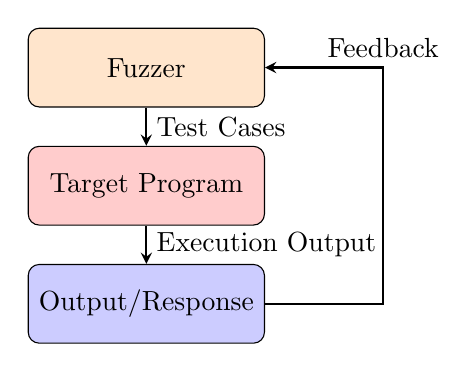
\begin{tikzpicture}[node distance=1.5cm]
                % Define styles for nodes and arrows
        \tikzstyle{box} = [rectangle, rounded corners, minimum width=3cm, minimum height=1cm, text centered, draw=black, fill=blue!20]
        \tikzstyle{fuzzer} = [rectangle, rounded corners, minimum width=3cm, minimum height=1cm, text centered, draw=black, fill=orange!20]
        \tikzstyle{target} = [rectangle, rounded corners, minimum width=3cm, minimum height=1cm, text centered, draw=black, fill=red!20]
        \tikzstyle{arrow} = [thick,->, >=stealth]
        \tikzstyle{title} = [rectangle, rounded corners, minimum width=5cm, text centered, draw=none, fill=none, font=\large\bfseries] 
    
        \node (fuzzer) [fuzzer] {Fuzzer};
        \node (target) [target, below of = fuzzer] {Target Program};
        \node (output) [box, below of = target] {Output/Response};

        % Arrows
        \draw  [arrow](fuzzer) -- (target) node[midway, right] {Test Cases};
        \draw [arrow] (target) -- (output) node[midway,right] {Execution Output};
        \draw [arrow] (output.east) --+(1.5,0) |- (fuzzer.east) node[midway, above] {Feedback};
    \end{tikzpicture}

\end{minipage}
&
\begin{minipage}{\dimexpr0.5\textwidth-2\tabcolsep}
\centering

    % Left Diagram - White Box Fuzzing
    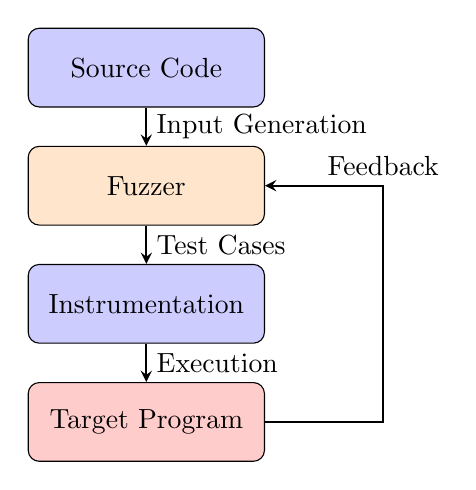
\begin{tikzpicture}[node distance=1.5cm]

        \tikzstyle{box} = [rectangle, rounded corners, minimum width=3cm, minimum height=1cm, text centered, draw=black, fill=blue!20]
        \tikzstyle{fuzzer} = [rectangle, rounded corners, minimum width=3cm, minimum height=1cm, text centered, draw=black, fill=orange!20]
        \tikzstyle{target} = [rectangle, rounded corners, minimum width=3cm, minimum height=1cm, text centered, draw=black, fill=red!20]
        \tikzstyle{arrow} = [thick,->, >=stealth]
        \tikzstyle{title} = [rectangle, rounded corners, minimum width=5cm, text centered, draw=none, fill=none, font=\large\bfseries]
        \node (source) [box] {Source Code};
        \node (fuzzer) [fuzzer, below of = source] {Fuzzer};
        \node (instr) [box, below of = fuzzer] {Instrumentation};
        \node (target) [target, below of = instr] {Target Program};

        % Arrows
        \draw  [arrow](source) -- (fuzzer) node[midway, right] {Input Generation};
        \draw  [arrow](fuzzer) -- (instr) node[midway, right] {Test Cases};
        \draw  [arrow](instr) -- (target) node[midway, right] {Execution};
        \draw  [arrow](target.east) -- +(1.5,0) |- (fuzzer.east) node[midway, above] {Feedback};

    \end{tikzpicture}
    
\end{minipage}

\\

\begin{minipage}[t]{\dimexpr0.5\textwidth-1\tabcolsep}
\captionof{figure}{Simplified black-box fuzzing process}
    \label{fig:black-box-testing}

\end{minipage}
&
\begin{minipage}[t]{\dimexpr0.5\textwidth-1 \tabcolsep}
\captionof{figure}{Simplified white-box fuzzing process}
\label{fig:white-box-testing}

\end{minipage}

\end{tabular*}

\subsubsection{Black Box Fuzzing}
\label{sec:black-box}
\textit{Black box fuzzing} (ref. \autoref{fig:black-box-testing}) is a software testing method that evaluates an application’s security and robustness by feeding it random or semi-random inputs without any knowledge of its internal workings—such as source code, data structures, or algorithms. This approach simulates an external attacker's perspective, enabling testers to discover vulnerabilities that might be exploited by malicious users in a real-world scenario.

The key characteristic of black-box fuzzing is its lack of insight into the internal design and logic of the software being tested. Instead, the focus is on the inputs and outputs of the application. Testers generate a wide variety of input data, often using automated tools or scripts, to gauge how the application responds. This can include testing edge cases, invalid inputs, or unexpected data formats to determine how robust the application is against improper use.

One of the main advantages of black-box fuzzing is its simplicity and ease of use. Since testers do not need to understand the details of the application’s code, they can quickly implement fuzzing without extensive knowledge of the underlying logic. This makes black-box fuzzing an attractive option for assessing third-party software or legacy applications where source code is not available.

Black-box fuzzing can be effective in identifying common security vulnerabilities, such as buffer overflows, input validation errors, and unexpected crashes. By observing how the application behaves with various inputs, testers can pinpoint areas of insecurity, allowing developers to focus their remedial efforts on the most critical issues.

Though black-box fuzzing offers valuable insights into application security, it does have some limitations. Specifically, the randomness of the generated inputs might not exercise all potential execution paths, leaving some vulnerabilities undiscovered. Furthermore, without knowledge of the internal code structure, it can be challenging to prioritize which vulnerabilities are more critical based on potential impact.

In conclusion, black-box fuzzing is an essential technique within the realm of software security testing. By simulating external attacks and evaluating the application solely based on its inputs and outputs, this method helps identify significant vulnerabilities that can compromise the application’s integrity. While it may lack the depth of white-box approaches, black-box fuzzing remains a crucial tool in the arsenal of security professionals, enabling them to enhance the overall security posture of applications in a comprehensive manner. \cite{godefroid_random_2007}

\subsubsection{White Box Fuzzing}
\label{sec:white-box}
\textit{White box fuzzing} (ref. \autoref{fig:white-box-testing}) is an advanced software testing technique that seeks to identify vulnerabilities and bugs within applications by utilizing an in-depth understanding of their internal structures and logic. Unlike traditional black-box testing methods, where testers approach the software without any knowledge of its internal workings, white-box fuzzing leverages access to the source code, algorithms, and data flows, allowing for a more targeted and effective analysis.

One of the primary benefits of white-box fuzzing is its ability to generate test inputs based on the actual paths and branches present in the code. By analyzing the control flow and data structures inherent to the application, white-box fuzzers can create specific input cases that exercise various execution paths. This targeted approach increases the likelihood of uncovering potential weaknesses, particularly in areas of the code that may be prone to errors or security vulnerabilities.

Additionally, white-box fuzzing often incorporates dynamic analysis. During the fuzzing process, the application is executed in a controlled environment, and its behavior is monitored in real-time. This provides valuable feedback on how the program reacts to the generated inputs, enabling the identification of unhandled cases that may lead to crashes, incorrect outputs, or security flaws.

Another critical feature of white-box fuzzing is coverage measurement. By measuring code coverage, testers can ensure that their input generation strategies are effective in exercising different paths within the software. This helps identify areas of the code that have not been adequately tested, enabling a more comprehensive examination of the program's reliability and security.

The primary objective of white-box fuzzing is to detect issues such as buffer overflows, null pointer dereferences, and other runtime errors that could compromise an application’s stability or allow for security breaches. By identifying these vulnerabilities early in the development process, organizations can address them proactively, ultimately enhancing the overall quality and security of their software.

In summary, white-box fuzzing is a powerful and efficient technique for software testing, combining knowledge of internal application structures with automated input generation and dynamic monitoring. This method significantly contributes to improving the robustness and security of software applications by exposing vulnerabilities that may be overlooked in traditional testing approaches.\cite{godefroid_random_2007}




\subsection{Dynamic Symbolic Execution}
\label{sec:dse}
\textit{Dynamic symbolic execution} (DSE) is a technique similar to white-box fuzzing, as it requires access to the source code. However, instead of requiring an actual input, it assumes that the variables are "symbolic," meaning that they do not possess a tangible value during execution of the program. Instead, it tracks the conditions encountered during runtime, generating constraints based on the symbolic variables. This facilitates a comprehensive examination of multiple program pathways, thereby aiding in the identification of anomalies that may result in unforeseen behaviour or security vulnerabilities.

After exploring a particular execution path, DSE employs constraint solvers to analyse the constraints collected during execution. These solvers determine concrete inputs that can satisfy the path constraints, allowing the generation of specific test cases to trigger particular code paths during subsequent executions.

By integrating DSE into white-box fuzzing, testers can automatically generate test cases that reliably expose bugs or vulnerabilities, such as buffer overflows or access violations. This allows for a more exhaustive testing process that can reveal flaws that traditional fuzzing techniques might overlook.

The synergy between DSE and white-box fuzzing promotes automated test generation and increases the coverage of tested paths, ultimately improving the software's reliability and security. It provides developers with concrete inputs that reproduce identified vulnerabilities, facilitating easier debugging and remediation.

In summary, dynamic symbolic execution significantly enhances the capabilities of white-box fuzzing by providing a structured, thorough, and automated approach to analyze program behavior. It helps identify and confirm vulnerabilities through the intelligent exploration of execution paths, making it a powerful tool in software testing and security analysis.

Let us proceed through the process of generating the path conditions (abbrv. PC) by employing the ensuing code snippet (\autoref{fig:code-snippet}). 
\begin{figure}[ht]
    \begin{lstlisting}[language=JavaScript, gobble=4, escapechar=@]
    function g(x) {
        if (x < 0){
            x=-x;
        }
        else {
            if (x === 0){
                x=1;
            }
            x = x + 1;
        }
        if (!(x >0)){
            x =-1;
        }
    }
    \end{lstlisting}
    \caption{A simple program}
    \label{fig:code-snippet}
\end{figure}


\subsection{SMT Solver}
\label{sec:smtsolver}

A \textit{satisfiability modulo theories }(SMT) Solver, is used to solve mathematical and logical problems. 

\section{Tech Stack}
\label{sec:tech}
In this section, we will delve into the inner workings of the expoSE framework, what tools it uses and their function within.


\subsection{Jalangi}
\label{sec:jalangi}

Jalangi2 is used in order to instrument the javascript code that is to be analyzed. 
\begin{figure}[ht]
    \begin{lstlisting}[language=JavaScript, gobble=4]
    J$.iids = {"8":[9,7,9,14],"9":[2,10,2,17],"10":[6,6,6,11]...,"nBranches":6}
    [...]
    x = J$.N(257, 'x', x, 4);
    if (J$.X1(345, J$.C(16, J$.B(10, '<', J$.R(89, 'x', x, 0), J$.T(97, 0, 22, false), 0)))) {
        J$.X1(121, x = J$.W(113, 'x', J$.U(18, '-', J$.R(105, 'x', x, 0)), x, 0));
    } else {
        [...]
    }
    [...]
    }

    \end{lstlisting}
    \caption{A simple program snippet, instrumented by JALANGI2}
    \label{fig:code-snippet}
\end{figure}
 
\subsection{Z3 SMT Solver}
\label{sec:z3}


ExpoSE uses the Z3 SMT Solver for solving the found path conditions of the analysed program. Developed by Microsoft, it has constant progress and improvements to its capabilities. 

\subsection{Z3Javascript}
\label{sec:z3js}

Z3Javascript is an extension for Z3 to generate JavaScript bindings to be used in ExpoSE.


\subsection{expoSE}
\label{sec:expose}
So, what exactly is this ominous "ExpoSE" we keep on talking about? 
In short, it is a DSE Framework for JavaScript, which allows almost any (explanation why almost see \autoref{sec:limits}), to be tested for reachability and bugs.

